\documentclass[../structural_economics_book.tex]{subfiles}
\begin{document}
\ifSubfilesClassLoaded{\setcounter{chapter}{15}}{}
\chapter{The Global Weight Matrix}\label{ch:16}
\chaptersubtitle{Center, Periphery, and the Spectral Structure of World Trade}
\begin{quote}
\textit{``Las ventajas del progreso t\'{e}cnico se han concentrado principalmente en los centros industriales, sin propagarse a la periferia del sistema econ\'{o}mico mundial en medida suficiente.''}\\[0.3em]
\textnormal{[``The advantages of technical progress have concentrated principally in the industrial centers, without propagating to the periphery of the world economic system in sufficient measure.'']}\\
\hfill --- Ra\'{u}l Prebisch, \textit{El desarrollo econ\'{o}mico de la Am\'{e}rica Latina y algunos de sus principales problemas} (1949)
% TODO-VERIFY: wording looks like a paraphrase of the 1949 study (CEPAL, Santiago); check against the original Spanish text and add page.
\end{quote}
\nocite{prebisch1949desarrollo}

\vspace{0.3em}

\begin{quote}
\textit{``Development depends not so much on finding optimal combinations for given resources and factors of production as on calling forth and enlisting for development purposes resources and abilities that are hidden, scattered, or badly utilized.''}\\
\hfill --- Albert O.\ Hirschman, \textit{The Strategy of Economic Development} (1958)
\end{quote}
\nocite{hirschman1958strategy}

\vspace{1em}

Part~V applies the framework to three scales: global (this chapter), national (Chapter~17), and individual (Chapter~18). At each scale, the same mathematics operates: the weight matrix $W$, the Perron eigenvector $\boldsymbol{\pi}$, the spectral gap $\Gamma$, and the formation model. What changes is the data.

This chapter takes $W^P_{\text{global}}$: the weight matrix of international trade, where countries are nodes and trade flows are edges. Its Perron vector measures how concentrated structural power is among countries --- Prebisch's center-periphery hypothesis, in one of its dimensions. Its spectral gap measures something else: how fast shocks mix across the world economy. The Economic Complexity Index \citep{hidalgo2009building} is a spectral object too, but of a different matrix, built from countries' export baskets rather than from bilateral trade. Hirschman's linkages are column and row sums of the Leontief inverse of the inter-country \emph{coefficient} matrix $A$, not of $W$.

Everything in Chapters~1--15 applies. The only difference is that $N$ is now 200 countries rather than 4 agents, and $W$ is estimated from trade data rather than assumed.


%% =====================================================================
\section{The Global Production Network}
\label{ch16:sec:global_WP}
%% =====================================================================

\subsection{From Bilateral Trade to the Weight Matrix}

\begin{definition}[Global Production Weight Matrix]\label{ch16:def:global_WP}
Let $K_{cc'}$ be the value (in USD) of country $c$'s imports from country $c'$, for $c \neq c'$. The \textbf{global production weight matrix} is $W^P = D^{-1}K$ with $D = \operatorname{diag}(K\ones)$:
\begin{equation}\label{ch16:eq:global_WP}
W^P_{cc'} = \frac{K_{cc'}}{\sum_{c''} K_{cc''}}.
\end{equation}
Entry $W^P_{cc'}$ is the share of country $c$'s imports that comes from country $c'$, so $W^P$ is row-stochastic. Two treatments of the diagonal must be distinguished:
\begin{itemize}
\item \emph{Imports only} (BACI, COMTRADE): $K_{cc} = 0$, so $W^P_{cc} = 0$.
\item \emph{Absorption shares} (inter-country input-output tables such as OECD ICIO): $K_{cc}$ is domestic purchases, so $W^P_{cc}$ is the domestic share of absorption, typically far larger than any import share. This $W^P$ is strongly diagonal, and its $\Gamma$ is much smaller than that of the imports-only matrix.
\end{itemize}
Every reported $\Gamma$ or $\boldsymbol{\pi}$ must state the source, year, country aggregation and diagonal treatment.
\end{definition}

For $N \approx 200$ countries and data from the BACI trade database (imports only) or an inter-country input-output table (absorption shares), $W^P_{\text{global}}$ is a row-stochastic matrix of that size. Aggregating countries into regions changes both $\Gamma$ and $\boldsymbol{\pi}$ (Exercise~\ref{ch16:ex:build}).

\begin{remark}[Properties of $W^P_{\text{global}}$ \illustrative]\label{ch16:prop:global_properties}
The numbers in this remark are illustrative; Exercise~\ref{ch16:ex:build} computes them from BACI.
\begin{enumerate}
\item \textbf{Not doubly stochastic.} The column sums of any row-stochastic $N \times N$ matrix average exactly $1$; here they vary by orders of magnitude, because large exporters appear in almost every country's import basket and small exporters in few. The column sum of the US is the sum, over importers, of the US share of their imports --- well above $1$; Bolivia's is well below $1$. The world does not depend on Bolivia the way Bolivia depends on the world.
\item \textbf{Core-periphery topology.} A dense core of 20--30 industrialized countries (high mutual trade) and a sparse periphery of 150+ countries (trade mostly with the core, rarely with each other).
\item \textbf{Concentrated Perron vector.} In our illustrative numbers the US has $\pi \approx 0.18$, China $0.15$ and Germany $0.08$, with the top 10 countries holding $\approx 65\%$ of structural power and $\pi_{\text{Bolivia}} \approx 0.0005$. Concentration is what $\Neff$ and $\Var(\boldsymbol{\pi})$ measure.
\item \textbf{The spectral gap measures frictions, not power.} A core-periphery structure in which everyone buys mainly from the core is close to rank one, and rank-one matrices have $\Gamma = 1$ for any $\boldsymbol{\pi}$. In frictionless gravity, every importer's shares equal the exporters' world shares $\mathbf{s}$: $W^P = \ones\mathbf{s}'$, with $\Gamma = 1$ and $\boldsymbol{\pi} = \mathbf{s}$, as concentrated as world exports. A measured $\Gamma$ below $1$ therefore reflects distance, trade costs and regional blocs --- how far the world is from anonymous market interaction (Chapter~1, Section~\ref{ch01:sec:conventions}) --- not how unequal power is (Proposition~\ref{ch06:prop:gap-power-independent}).
\end{enumerate}
\end{remark}

\begin{vizpanel}{The global $W^P$: a $10 \times 10$ schematic}
\begin{center}
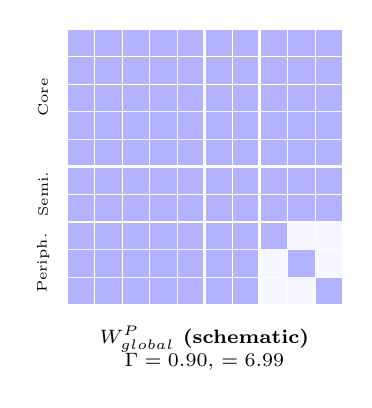
\begin{tikzpicture}[scale=1]
\def\N{10}
\def\s{0.35}
%% Core countries (1-5): dense mutual trade
%% Semi-periphery (6-7): moderate links to core
%% Periphery (8-10): sparse, mostly to core
\foreach \i in {1,...,\N} {
  \foreach \j in {1,...,\N} {
    \pgfmathparse{
      (\i<=5 && \j<=5) ? 65 :
      (\i<=5 && \j>5 && \j<=7) ? 25 :
      (\i<=5 && \j>7) ? 5 :
      (\i>5 && \i<=7 && \j<=5) ? 45 :
      (\i>5 && \i<=7 && \j>5 && \j<=7) ? 35 :
      (\i>5 && \i<=7 && \j>7) ? 8 :
      (\i>7 && \j<=5) ? 50 :
      (\i>7 && \j>5 && \j<=7) ? 10 :
      (\i>7 && \j>7 && \i==\j) ? 30 :
      3
    }
    \edef\bp{\pgfmathresult}
    \fill[blue!\bp, draw=white, line width=0.08pt]
      ({(\j-1)*\s}, {(\N-\i)*\s}) rectangle +(\s,\s);
  }
}
\node[font=\tiny, black, rotate=90] at (-0.3, {7.5*\s}) {Core};
\node[font=\tiny, black, rotate=90] at (-0.3, {4*\s}) {Semi.};
\node[font=\tiny, black, rotate=90] at (-0.3, {1.5*\s}) {Periph.};
\draw[white, thick] (0, {5*\s}) -- ({\N*\s}, {5*\s});
\draw[white, thick] (0, {3*\s}) -- ({\N*\s}, {3*\s});
\draw[white, thick] ({5*\s}, 0) -- ({5*\s}, {\N*\s});
\draw[white, thick] ({7*\s}, 0) -- ({7*\s}, {\N*\s});

\node[below, font=\scriptsize\bfseries] at ({5*\s}, -0.15) {$W^P_{\text{global}}$ (schematic)};
\node[below, font=\scriptsize] at ({5*\s}, -0.5) {$\Gamma = 0.90$, $\Neff = 6.99$};
\end{tikzpicture}
\qquad
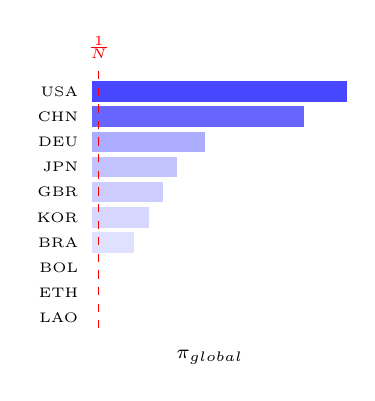
\begin{tikzpicture}[scale=1]
%% Power bars for 10 "countries"
\foreach \k/\val/\lab in {1/0.18/USA,2/0.15/CHN,3/0.08/DEU,4/0.06/JPN,5/0.05/GBR,6/0.04/KOR,7/0.03/BRA,8/0.0005/BOL,9/0.0004/ETH,10/0.0003/LAO} {
  \pgfmathparse{\val*400}
  \edef\bp{\pgfmathresult}
  \fill[blue!\bp] (0, {(10-\k)*0.32}) rectangle ({\val*18}, {(10-\k)*0.32+0.26});
  \node[font=\tiny, left] at (-0.05, {(10-\k)*0.32+0.13}) {\lab};
}
\draw[red, dashed, thin] ({0.005*18}, 0) -- ({0.005*18}, 3.3);
\node[font=\tiny, red, above] at ({0.005*18}, 3.3) {$\frac{1}{N}$};
\node[below, font=\scriptsize\bfseries] at (1.5, -0.15) {$\boldsymbol{\pi}_{\text{global}}$};
\end{tikzpicture}
\end{center}
\vspace{-0.5em}
\small Left: schematic global $W^P$ (row-normalized cell values in \texttt{code/ch16.py}). The upper-left block (core) is bright: dense mutual trade. The lower-right (periphery) is dark except for column entries toward the core: the periphery depends on the core, not on each other. The lower-left rectangle is brighter than the upper-right: asymmetric dependence. This hub structure is close to rank one, so its spectral gap is \emph{large} ($\Gamma = 0.90$): everyone mixes quickly through the core. Its power is concentrated: the five core countries hold $0.163$ each, the periphery $0.016$ each. Right: an illustrative Perron vector for 200 countries. The dashed red line marks $1/N = 0.005$. The US alone has 36 times the ``fair share'' of structural power. Bolivia is barely visible.
\end{vizpanel}


\subsection{The Global Leontief Inverse}

\begin{definition}[Global Leontief Inverse and Linkages]\label{ch16:def:global_leontief}
Let $A$ be the inter-country input-output coefficient matrix, with the Chapter~1 convention: $a_{cc'}$ is the input from country $c'$ needed per unit of country $c$'s output (row $c$ is $c$'s recipe), and $\y = A'\y + \mathbf{d}$. The \textbf{global Leontief inverse} is $L = (I - A')^{-1}$, which exists with $L \geq I$ when $\rho(A) < 1$. Entry $\ell_{cc'}$ is the gross output generated in country $c$ by a unit of final demand for country $c'$'s output, including all rounds of indirect effects through the global supply chain.
\begin{enumerate}
\item Country $c'$'s \textbf{backward linkage} is $BL_{c'} = \sum_c \ell_{cc'}$ (column sum): the total gross output generated by one unit of final demand for $c'$. High $BL$: $c'$ uses many intermediate inputs, domestic or foreign.
\item Country $c$'s \textbf{forward linkage} is $FL_c = \sum_{c'} \ell_{cc'}$ (row sum): how much of $c$'s output is required, directly and indirectly, when every country's final demand rises by one unit. (The Ghosh supply-side inverse is the usual alternative for forward linkages.)
\item The \textbf{key sector} \citep{rasmussen1956studies} has both $BL > \bar{BL}$ and $FL > \bar{FL}$: it generates demand upstream AND supplies inputs downstream.
\end{enumerate}
Since $L \geq I$, every $BL$ and $FL$ is at least $1$, and $\bar{BL} = \bar{FL}$ (both equal the sum of all entries of $L$ divided by $N$). These indices must be computed from $A$: for the row-stochastic $W^P$, $(I - \gamma W^P)^{-1}\ones = \ones/(1-\gamma)$, so every row sum would be the same.
\end{definition}

\begin{example}[Global Linkages \illustrative]\label{ch16:ex:global_linkages}
Illustrative country-level linkages, of the kind one obtains by aggregating an inter-country input-output table to countries (Bolivia and Ethiopia are not separate economies in OECD ICIO, which places them in the Rest of the World; for them a table such as Eora would be needed):

\begin{center}
\begin{tabular}{lccl}
\toprule
Country & $BL$ & $FL$ & Type \\
\midrule
United States & 2.45 & 1.98 & High/High: key sector (global hub) \\
China & 2.68 & 2.31 & High/High: manufacturing hub \\
Germany & 2.51 & 2.12 & High/High: machinery hub \\
Japan & 2.33 & 1.85 & High/High \\
Bolivia & 1.28 & 1.12 & Low/Low: peripheral enclave \\
Ethiopia & 1.15 & 1.08 & Low/Low \\
\midrule
Average (all economies) & 1.85 & 1.85 & equal by construction \\
\bottomrule
\end{tabular}
\end{center}

The center has $BL$ and $FL$ both above average: it generates demand AND supplies inputs. The periphery has both below average: its demand doesn't propagate, and its output isn't widely used. Bolivia's $BL = 1.28$ means that one dollar of final demand for Bolivian output generates only \$1.28 of gross output worldwide, including the dollar itself (vs.\ \$2.68 for China): Bolivian production uses few intermediate inputs per unit of output.
\end{example}


%% =====================================================================
\section{Economic Complexity as Spectral Measurement}
\label{ch16:sec:ECI}
%% =====================================================================

\subsection{From Trade Data to the Specialization Matrix}

The Economic Complexity Index (ECI) is a dimensionality-reduction method that extracts the leading non-trivial spectral structure from the country--product export matrix. It uses no bilateral information --- who sells to whom --- so it is not a function of $W^P_{\text{global}}$; it is a spectral summary of a different matrix, built from what each country exports.

\begin{definition}[Specialization Matrix and RCA]\label{ch16:def:RCA}
Let $X_{cp}$ be the export value of product $p$ from country $c$. The \textbf{Revealed Comparative Advantage} is:
\begin{equation}\label{ch16:eq:RCA}
R_{cp} = \frac{X_{cp}/X_c}{X_p/X},
\end{equation}
where $X_c = \sum_p X_{cp}$, $X_p = \sum_c X_{cp}$, and $X = \sum_{c,p} X_{cp}$. A country has comparative advantage in product $p$ if $R_{cp} > 1$. The binary specialization matrix: $M_{cp} = \mathbf{1}[R_{cp} \geq 1]$.
\end{definition}

\begin{definition}[The Proximity Matrix and Product Space]\label{ch16:def:proximity}
The \textbf{proximity} between products $p$ and $p'$ is:
\begin{equation}\label{ch16:eq:proximity}
\phi_{pp'} = \frac{\sum_c M_{cp}M_{cp'}}{\max(M_p, M_{p'})},
\end{equation}
where $M_p = \sum_c M_{cp}$ is the ubiquity of product $p$. The \textbf{product space} is the network with products as nodes and $\phi_{pp'}$ as edge weights.
\end{definition}

The product space is a network of \emph{capability similarity} between products: two products are close when the same countries tend to export both. It is not an input-output network, and it is not $W^P$ at the product level. Its topology --- dense core of machinery/chemicals/electronics, sparse periphery of raw materials --- was first mapped for about 775 products \citep{hidalgo2007product} and is now drawn over 5,000+.


\subsection{The ECI as the Second Eigenvector}

\begin{definition}[Economic Complexity Index]\label{ch16:def:ECI}
Define the country-country matrix:
\begin{equation}\label{ch16:eq:Mcc}
\tilde{M}_{cc'} = \sum_p \frac{M_{cp}M_{c'p}}{M_c \cdot M_p},
\end{equation}
where $M_c = \sum_p M_{cp}$ is diversity. $\tilde{M}_{cc'}$ measures the similarity between countries $c$ and $c'$ based on their shared products, weighted by product ubiquity. This matrix is row-stochastic.

The \textbf{ECI} is the second eigenvector of $\tilde{M}$:
\begin{equation}\label{ch16:eq:ECI}
\tilde{M}\mathbf{v}_2 = \lambda_2 \mathbf{v}_2, \qquad \text{ECI}_c = \frac{v_{2,c} - \text{mean}(v_2)}{\text{stdev}(v_2)}.
\end{equation}
The first eigenvector is trivial ($\ones$, since $\tilde{M}$ is row-stochastic). The second eigenvector is the leading non-trivial spectral structure of the export matrix; its sign is chosen so that ECI correlates positively with diversity.
\end{definition}

\begin{proposition}[Spectral Facts About $\tilde{M}$]\label{ch16:thm:ECI_gamma}
Let $D_c = \operatorname{diag}(M_c)$ and $D_p = \operatorname{diag}(M_p)$, with all diversities and ubiquities positive. Then:
\begin{enumerate}
\item $\tilde{M} = D_c^{-1}MD_p^{-1}M'$ is row-stochastic, and its eigenvalues are real and lie in $[0, 1]$: they are the squared singular values of $S = D_c^{-1/2}MD_p^{-1/2}$.
\item The left Perron vector of $\tilde{M}$ is proportional to diversity: $\boldsymbol{\pi}(\tilde{M})_c = M_c/\sum_{c'}M_{c'}$. In the ``power'' reading of this book, the structural power of a country in $\tilde{M}$ is its diversity share.
\item ECI is a $z$-score, so its cross-country variance is $1$ by construction and carries no information about inequality.
\end{enumerate}
\end{proposition}

\begin{proof}
(1) Row sums: $\sum_{c'}\tilde{M}_{cc'} = \sum_p \frac{M_{cp}}{M_c}\sum_{c'}\frac{M_{c'p}}{M_p} = 1$. Also $\tilde{M} = D_c^{-1/2}(SS')D_c^{1/2}$ is similar to the positive semidefinite matrix $SS'$, whose eigenvalues are squared singular values; since $\tilde{M}$ is stochastic they are at most $1$. (2) For each $c'$,
\[
\textstyle\sum_c M_c\tilde{M}_{cc'} = \sum_p \frac{M_{c'p}}{M_p}\sum_c M_{cp} = \sum_p M_{c'p} = M_{c'}.
\] (3) By definition~\eqref{ch16:eq:ECI}. \texttt{code/ch16.py} checks (1)--(2) numerically.
\end{proof}

Interpretation: ECI orders countries along the principal axis of differentiation in export baskets. High ECI = diverse, complex exports (machinery, chemicals, pharmaceuticals). Low ECI = concentrated, simple exports (oil, minerals, raw agriculture). $\lambda_2(\tilde{M})$ close to $1$ means that axis is strong (countries split sharply into two groups of baskets); close to $0$ means baskets are similar. The gap $1 - \lambda_2(\tilde{M})$ is the spectral gap of $\tilde{M}$, a different matrix from $W^P_{\text{global}}$; it says nothing about the integration of world trade.

\begin{intuition}[What the ECI measures, in this book's language]
The ECI measures where a country sits on the second eigenvector of the export-similarity matrix $\tilde{M}$ --- the axis that captures the most information about who exports what. A country with $\text{ECI} > 0$ exports what the diversified core exports; a country with $\text{ECI} < 0$ exports what the periphery exports. Its link to power is indirect: in $\tilde{M}$ itself, power is diversity.

Japan is at or near the top of the ranking: diversified and complex. Bolivia is in the lower part: concentrated and simple. The gap between them is a property of export baskets, which shapes --- but is not the same thing as --- the country's position in $W^P_{\text{global}}$.
\end{intuition}


\subsection{ECI Predicts Growth: A Structural Explanation}

\begin{empiricalresult}[ECI Predicts Growth]\label{ch16:prop:ECI_growth}
ECI predicts future growth of GDP per capita, controlling for current income \citep{hidalgo2009building,hausmann2014atlas}.
\end{empiricalresult}

\begin{conjecture}[A Structural Explanation]\label{ch16:conj:ECI_growth}
The predictive power of ECI works through three channels:
\begin{enumerate}
\item High ECI goes with stronger domestic inter-sectoral linkages, so shocks and demand propagate across sectors (Chapter~3); this should show up as a higher domestic $\Gamma(W^P)$ and higher multipliers computed from $A$.
\item High ECI goes with a diverse product portfolio, hence more independent signals in $W^I$ and a higher $\Neff$ (Chapter~8).
\item High ECI goes with a dense position in the product space, hence many feasible diversification paths (Chapter~13).
\end{enumerate}
\end{conjecture}

The standard explanation is that ECI proxies for human capital and institutions. The conjecture is that it also proxies for the integration of the domestic production network. Unlike the standard explanation, this one is testable with national input-output tables: compute domestic $\Gamma$ and multipliers and check whether they mediate the ECI--growth relation (Exercise~\ref{ch16:ex:bound}).


%% =====================================================================
\section{ECI and Inequality}
\label{ch16:sec:inequality}
%% =====================================================================

\begin{empiricalresult}[ECI and Inequality]\label{ch16:prop:ECI_inequality}
Countries with high ECI have lower income inequality (Gini), controlling for GDP per capita \citep[who report robustness across specifications and data sources]{hartmann2017linking}.
\end{empiricalresult}

\begin{remark}[What the framework does and does not explain]\label{ch16:thm:ECI_inequality}
It is tempting to explain this association with a ``spectral bound'': high ECI $\Rightarrow$ high $\Gamma$ $\Rightarrow$ low $\Var(\boldsymbol{\pi})$ $\Rightarrow$ low inequality. That chain fails at its second link. There is no bound of $\Var(\boldsymbol{\pi})$ by $\Gamma$: the matrix $W = \gamma\,\ones\boldsymbol{\pi}' + (1-\gamma)I$ has $\Gamma = \gamma$ and Perron vector $\boldsymbol{\pi}$ for \emph{any} $\boldsymbol{\pi}$ (Proposition~\ref{ch06:prop:gap-power-independent}); at $\gamma = 1$ a near-dictatorship has $\Gamma = 1$. The chain also mixes levels: $\boldsymbol{\pi}$ of $W^P_{\text{global}}$ describes inequality \emph{between} countries, while the Gini coefficient describes inequality \emph{within} them.

What the framework does supply is the exact link between \emph{domestic} power concentration and distributional loss under the allocation rule of Chapter~7: $L_{\text{power}} = \frac{\kappa N}{2}\Phi^2\Var(\boldsymbol{\pi})$, with $\Var(\boldsymbol{\pi}) = \frac{1}{N}\big(\frac{1}{\Neff} - \frac{1}{N}\big)$. A structural explanation of the ECI--inequality association therefore has to run through the domestic power vector --- for example, a diversified production structure spreading $\boldsymbol{\pi}$ across more sectors and groups (higher $\Neff$) --- and that is an empirical hypothesis, testable with the diagnostics of Chapter~17.
\end{remark}

\begin{prebisch}[Fajnzylber's casillero vac\'{i}o]
In \citeyear{fajnzylber1990industrializacion}, Fernando Fajnzylber published ``Industrializaci\'{o}n en Am\'{e}rica Latina: de la `caja negra' al `casillero vac\'{i}o'\,'' documenting that no Latin American country occupied the cell of a $2 \times 2$ table that combines high growth with equity --- the ``casillero vac\'{i}o'' (empty box). Several countries outside the region, such as South Korea, did occupy it. The empty box is defined in the space of \emph{growth} $\times$ \emph{equity}, not of complexity $\times$ inequality.

Chapter~17 develops Fajnzylber's argument as its case study. Its link to this chapter is the empirical association above: both high growth (Empirical Result~\ref{ch16:prop:ECI_growth}) and lower inequality (Empirical Result~\ref{ch16:prop:ECI_inequality}) go with high ECI, which is why raising complexity --- changing the production structure through the operators of Chapter~15 --- is the structuralist route into the box.
\end{prebisch}

\begin{vizpanel}{Complexity and inequality: a schematic}
\begin{center}
\begin{tikzpicture}[scale=1]
\draw[->] (0,0) -- (7,0) node[right, font=\small] {ECI};
\draw[->] (0,0) -- (0,4.2) node[above, font=\small] {Gini};

%% Schematic scatter (anonymous points, illustrative)
\foreach \cx/\cy in {5.8/0.9, 5.2/1.0, 4.5/1.3, 4.8/1.9, 4.0/1.1, 3.8/1.6, 3.5/2.0, 3.0/2.6, 2.5/2.3, 2.8/3.4, 2.0/2.9, 1.5/2.6, 1.2/1.9, 1.0/2.2, 0.8/3.0, 2.2/1.7} {
  \fill[blue!50!black] (\cx, \cy) circle (1.5pt);
}
%% Least-squares line through the schematic points (code/ch16.py)
\draw[red!70!black, thick, dashed] (0.5, 2.87) -- (6.3, 0.93);
\node[font=\scriptsize, red!70!black, right] at (6.3, 0.93) {fitted line};
\end{tikzpicture}
\end{center}
\vspace{-0.5em}
\small Schematic only (illustrative, anonymous points): the negative association between complexity and inequality documented by \citet{hartmann2017linking}. There is no spectral ``fence'': the dispersion around the line is large, and nothing in the framework rules out low-complexity, low-inequality outcomes. Fajnzylber's casillero vac\'{i}o lives in a different plane, growth $\times$ equity (Chapter~17).
\end{vizpanel}


%% =====================================================================
\section{Relatedness and the Global $W^P$ Dynamics}
\label{ch16:sec:relatedness}
%% =====================================================================

\subsection{The Principle of Relatedness as Global Path Dependence}

\begin{definition}[Relatedness Density]\label{ch16:def:relatedness}
Country $c$'s \textbf{relatedness density} to product $p$ is:
\begin{equation}\label{ch16:eq:relatedness}
\omega_{cp} = \frac{\sum_{p'} M_{cp'}\phi_{pp'}}{\sum_{p'}\phi_{pp'}}.
\end{equation}
This is the fraction of related products that $c$ already produces. High $\omega_{cp}$: country $c$ has the capabilities to produce $p$. Low $\omega_{cp}$: the capabilities are missing.
\end{definition}

\begin{stylizedfact}[The Principle of Relatedness]\label{ch16:prop:relatedness_global}
The probability that country $c$ develops RCA in product $p$ (enters the product) is increasing in $\omega_{cp}$ \citep{hidalgo2007product}. Countries diversify into products related to their current exports, not into random products.
\end{stylizedfact}

This is what the path-dependence conjecture of Chapter~13 predicts when edge creation is proximity-dominated ($p_1 \gg p_2, p_3$): new edges form near existing edges. The global consequence: countries on the dense core of the product space (high $\omega_{cp}$ for many products) diversify rapidly and raise their ECI; countries on the sparse periphery (low $\omega_{cp}$ for core products) diversify slowly or not at all, and remain at low ECI.

\begin{example}[Relatedness Density: Bolivia vs.\ South Korea \illustrative]\label{ch16:ex:relatedness}
\begin{center}
\begin{tabular}{lcc}
\toprule
Target product & $\omega_{\text{Bolivia}}$ & $\omega_{\text{Korea}}$ \\
\midrule
Lithium batteries & 0.04 & 0.52 \\
Pharmaceutical intermediates & 0.03 & 0.41 \\
Automotive parts & 0.02 & 0.68 \\
Processed food machinery & 0.08 & 0.45 \\
\midrule
Average (all core products) & 0.06 & 0.55 \\
\bottomrule
\end{tabular}
\end{center}

Korea's average relatedness to core products is 9 times Bolivia's. (Korea already has comparative advantage in several of these products; its column illustrates the density of a country inside the core.) Korea can diversify into products like these with high probability; Bolivia cannot, without the sequenced operators from Chapter~15 (information $\to$ institutions $\to$ education $\to$ infrastructure $\to$ industrial policy).
\end{example}


%% =====================================================================
\section{The Terms of Trade: A Spectral Conjecture}
\label{ch16:sec:terms}
%% =====================================================================

\begin{conjecture}[Prebisch--Singer as a Spectral Hypothesis]\label{ch16:thm:prebisch_singer}
Apply the allocation rule of Chapter~7 (Proposition~\ref{ch07:prop:allocation-rule}) to countries, reading $\boldsymbol{\pi}(W^P_{\text{global}})$ as bargaining weights (an assumption, not a result):
\begin{equation}\label{ch16:eq:global_bargaining}
x_c^* = \frac{\Omega_{\text{global}}}{N} + \Big(\pi_c(W^P_{\text{global}}) - \frac{1}{N}\Big)\Phi.
\end{equation}
Countries with high structural power ($\pi_c > 1/N$) receive more than an equal share of global output; countries with low power ($\pi_c < 1/N$) receive less. The conjecture is that the terms-of-trade deterioration of primary exporters is the dynamic counterpart: as the global $W^P$ evolves (Chapter~13), the core's $\pi$ rises (the core adds dense linkages) and the periphery's $\pi$ falls.
\end{conjecture}

Two caveats keep this a conjecture. First, $x_c$ is a share of output, not a relative price: a theory of the terms of trade needs prices, which~\eqref{ch16:eq:global_bargaining} does not contain. Second, Prebisch's own mechanisms are different and more specific: low income elasticities of demand for primary goods, and asymmetric behaviour of wages and prices over the cycle, so that technical progress in the center is absorbed as higher incomes and in the periphery as lower prices. The empirical record on the long-run trend is itself debated \citep{grilli1988primary,harvey2010prebisch,arezki2014testing}. A spectral version would have to derive relative prices from $W$ and show that they move with $\boldsymbol{\pi}$.

\begin{example}[Bolivia's Terms of Trade \illustrative]\label{ch16:ex:bot_terms}
Bolivia's commodity export prices (gas, tin, zinc, soy) have experienced long-run terms-of-trade deterioration interspersed with commodity booms (1970s, 2003--2014). Because $W^P_{\text{global}}$ is built from trade \emph{values}, a price boom does change it: Bolivia's shares in its partners' imports rise, and so does $\pi_{\text{Bolivia}}$. But it changes only the weights on existing edges --- no new products, no new partners --- and the gain reverses with prices. After booms, $x_{\text{Bolivia}}$ returns toward the pre-boom trajectory.

The gas nationalization of 2006 rerouted gas revenue from MNCs to the treasury --- a fiscal linkage --- but it did not add cross-sector domestic production linkages. Illustratively, Bolivia's ECI stood near $-0.85$ in 2006 and $-0.80$ in 2018: twelve years of gas revenue redistributed through fiscal channels, almost no change in the export structure.
\end{example}


%% =====================================================================
\section{The Three Networks at Global Scale}
\label{ch16:sec:three_global}
%% =====================================================================

The global economy has three networks, just as the domestic economy does.

\begin{remark}[Global Three-Network Structure]\label{ch16:prop:three_global}
\begin{enumerate}
\item $W^P_{\text{global}}$: the trade/production network. Measured by ICIO, BACI, or COMTRADE data. Core-periphery topology. (ECI is not computed from it, but from export baskets.)

\item $W^I_{\text{global}}$: the global information network. Measured (imperfectly) by media flows, academic citation patterns, policy diffusion. Hub-spoke topology centered on the US and Europe. The Washington Consensus as DeGroot equilibrium (Chapter~8). $\Neff$ of global economic policy, counting institutions as nodes: illustratively 3--5 (IMF, World Bank, US Treasury, ECB, a few think tanks).

\item $W^U_{\text{global}}$: the global utility network. Harder to measure. Includes foreign aid (revealed altruism), migration patterns (revealed social bonds), and cultural consumption (whose stories do you watch?). Also hub-spoke, correlated with $W^I$.
\end{enumerate}

The three networks are \textbf{aligned at the global scale}: the countries that are central in $W^P$ (trade hubs) are also central in $W^I$ (information hubs) and $W^U$ (cultural hubs). If the three layers are defined on the same node set (countries), this alignment reinforces the concentration of the composite Perron eigenvector (Chapter~5): the center is powerful in all three dimensions simultaneously.
\end{remark}

\begin{keyinsight}
The global spectral structure tells the same story at all three layers. $W^P$: the center produces the goods. $W^I$: the center produces the ideas. $W^U$: the center produces the culture. The periphery consumes all three and produces the raw materials. The Perron eigenvector is aligned across layers. Reducing that concentration --- raising $\Neff$ of the global composite --- is a distributional objective, separate from integration: the world is already highly integrated through its core ($\Gamma$ is high in a hub structure), and more integration on the same hub structure leaves power where it is. The current structure reproduces itself through the formation model (Chapter~10): peripheral preferences are formed under a $W^I$ that transmits center consumption patterns and economic doctrines. The formation loop operates at the global scale exactly as it does at the domestic scale.
\end{keyinsight}


%% =====================================================================
\section{Summary}
\label{ch16:sec:summary}
%% =====================================================================

\begin{enumerate}
\item The \textbf{global production weight matrix} $W^P_{\text{global}} = D^{-1}K$ is estimated from trade data; its values depend on the source, year, aggregation and diagonal treatment. Its column sums average $1$ and vary by orders of magnitude; its Perron vector is concentrated (illustratively $\pi_{\text{US}} \approx 0.18$, $\pi_{\text{Bolivia}} \approx 0.0005$).

\item A core-periphery hub structure has a \emph{large} spectral gap (the schematic has $\Gamma = 0.90$; frictionless gravity has $\Gamma = 1$). $\Gamma$ measures trade frictions and mixing; power concentration is measured by $\boldsymbol{\pi}$, $\Neff$ and $\Var(\boldsymbol{\pi})$.

\item The \textbf{ECI} is the second eigenvector of the export-similarity matrix $\tilde{M}$, not a function of $W^P_{\text{global}}$. $\tilde{M}$ has real eigenvalues in $[0,1]$ and a Perron vector proportional to diversity. ECI predicts growth and lower inequality empirically; the channels through domestic integration and domestic power are conjectures, and no spectral bound links $\Gamma$ to inequality.

\item \textbf{Relatedness density} is the empirical counterpart of proximity-dominated edge creation (Chapter~13). Countries on the dense core diversify rapidly; countries on the sparse periphery are locked in. Linkages ($BL$, $FL \geq 1$) come from the coefficient matrix $A$, not from $W$.

\item The \textbf{Prebisch--Singer hypothesis} has a spectral version --- the core's $\pi$ rises as the global $W^P$ evolves --- that remains a conjecture until relative prices are derived from $W$. The three global networks are \textbf{aligned}: the center dominates production, information, and culture simultaneously.
\end{enumerate}


%% =====================================================================
\section{Exercises}
\label{ch16:sec:exercises}
%% =====================================================================

\begin{enumerate}[label=\textbf{16.\arabic*}, leftmargin=3em]

\item \textbf{Build the global $W^P$.}\label{ch16:ex:build} Using BACI trade data (available at \texttt{cepii.fr}):
\begin{enumerate}
\item Download bilateral trade data for 2018. Keep all countries, and also aggregate to 50 countries (rest of world as one node).
\item Construct $W^P_{cc'}$ (Definition~\ref{ch16:def:global_WP}). Verify row-stochasticity.
\item Compute column sums. Which country has the largest? Smallest?
\item Compute $\boldsymbol{\pi}$ (power iteration, Appendix~6A). Plot $\pi_c$ vs.\ GDP per capita. What is the correlation?
\item Compute $\Gamma$ and $\Neff$ for the full and the 50-country matrix. How much does aggregation change each? Compare $\Gamma$ with the frictionless-gravity benchmark $\ones\mathbf{s}'$ ($\Gamma = 1$), where $\mathbf{s}$ is world export shares, and $\boldsymbol{\pi}$ with $\mathbf{s}$.
\end{enumerate}

\item \textbf{Compute the ECI.} Using the Atlas of Economic Complexity (\url{atlas.cid.harvard.edu}) or OEC (\texttt{oec.world}):
\begin{enumerate}
\item Download the ECI ranking for 2018. Identify the top 10 and bottom 10.
\item Plot ECI vs.\ GDP per capita. What is the correlation? Is it stronger or weaker than $\pi_c$ vs.\ GDP per capita from Exercise~16.1?
\item Plot ECI vs.\ Gini coefficient. Is the low-ECI, low-Gini quadrant sparsely populated? (This is not Fajnzylber's casillero vac\'{i}o, which is defined in growth $\times$ equity space; see Chapter~17.)
\item Where is Bolivia? Where is South Korea? What is the ECI gap?
\end{enumerate}

\item \textbf{Relatedness density.} Using OEC product-space data:
\begin{enumerate}
\item Compute Bolivia's relatedness density to: lithium batteries, processed food, pharmaceutical intermediates.
\item Compare with Chile, Peru, and Colombia.
\item Which country has the highest average relatedness to core products? Why?
\item Using Chapter~15's sequencing framework: what operator sequence would Bolivia need to reach $\omega > 0.3$ for lithium batteries?
\end{enumerate}

\item \textbf{Prebisch-Singer.} Download Bolivia's terms-of-trade index (World Bank WDI or CEPAL):
\begin{enumerate}
\item Plot the terms-of-trade index, 1960--2023.
\item Identify the commodity booms (1970s, 2003--2014). During booms: did Bolivia's ECI change?
\item Using BACI, recompute $\pi_{\text{Bolivia}}$ for a boom year and a bust year, first with current values and then with trade valued at constant (base-year) prices. How much of the change in $\pi_{\text{Bolivia}}$ is a price effect and how much a change in quantities and partners?
\end{enumerate}

\item \textbf{Global $W^I$.} Use data on academic citations (Scopus) or media reach (Reuters, AP, AFP) to estimate a proxy for $W^I_{\text{global}}$:
\begin{enumerate}
\item Construct a $20 \times 20$ matrix where $W^I_{cc'}$ is the share of academic citations in country $c$ that cite papers from country $c'$.
\item Compute $\boldsymbol{\pi}^I$. Which countries have the highest epistemic power?
\item Compute $N_{\text{eff}}$. How many ``independent voices'' shape the global academic consensus?
\item Compare $\boldsymbol{\pi}^I$ with $\boldsymbol{\pi}^P$ (from Exercise~16.1). Are they correlated? What does alignment mean for the composite power vector?
\end{enumerate}

\item \textbf{Integration, power and inequality.}\label{ch16:ex:bound} For 30--50 countries with national input-output tables (OECD ICIO):
\begin{enumerate}
\item Compute the domestic $\Gamma_c$ and $\Neff$ of the domestic $W^P = D^{-1}A$ for each country.
\item Show, by constructing $W = \gamma\,\ones\boldsymbol{\pi}' + (1-\gamma)I$, that no function of $\Gamma$ alone can bound $\Var(\boldsymbol{\pi})$.
\item Regress the Gini coefficient on ECI, then add $\Gamma_c$ and $\Neff$. Which, if any, mediates the ECI--inequality association of \citet{hartmann2017linking}?
\item Which countries have much lower inequality than their complexity would predict? What do they have in common?
\end{enumerate}

\item \textbf{Bolivia's structural position.} Synthesize all the data from this chapter's exercises:
\begin{enumerate}
\item Bolivia's $\pi_{\text{global}}$, ECI, relatedness density to core products, terms-of-trade trajectory, and $W^I$ position.
\item Using the operator-design framework of Chapter~15: design a 20-year structural transformation plan for Bolivia. Which operators, in what sequence, targeting which products?
\item Estimate the cost (order of magnitude) and the expected $\Delta$ECI, $\Delta\Gamma$, $\Delta$Gini.
\item Is the plan politically feasible given Bolivia's current coalition structure (Chapter~14)?
\end{enumerate}
\end{enumerate}


%% =====================================================================
\newpage
\section*{Mathematical Appendices}
\addcontentsline{toc}{section}{Mathematical Appendices}
%% =====================================================================


\subsection*{Appendix 16A: The ECI as a Spectral Method}
\addcontentsline{toc}{subsection}{Appendix 16A: ECI as Spectral Method}
\label{ch16:app:ECI}

\paragraph{Derivation.} Start with the binary specialization matrix $M$ ($C \times P$). Define diversity $M_c = \sum_p M_{cp}$ and ubiquity $M_p = \sum_c M_{cp}$. The coupled equations:
\begin{equation}
K_c = \frac{1}{M_c}\sum_p M_{cp}K_p, \qquad K_p = \frac{1}{M_p}\sum_c M_{cp}K_c.
\end{equation}

Substituting: $K_c = \sum_{c'} \tilde{M}_{cc'} K_{c'}$ where $\tilde{M}_{cc'} = \sum_p M_{cp}M_{c'p}/(M_cM_p)$. The solutions are the eigenvectors of $\tilde{M}$. Since $\tilde{M}$ is row-stochastic, the first eigenvector is $\ones$ (trivial). The ECI is the second eigenvector, Z-score normalized.

\paragraph{Connection to SVD.} Let $S = D_c^{-1/2}MD_p^{-1/2}$ with SVD $S = U\Sigma V'$. Then $\tilde{M} = D_c^{-1}MD_p^{-1}M' = D_c^{-1/2}(SS')D_c^{1/2} = D_c^{-1/2}U\Sigma^2U'D_c^{1/2}$, so the eigenvalues of $\tilde{M}$ are the squared singular values of $S$ and its right eigenvectors are $D_c^{-1/2}U$. The ECI is therefore, up to $z$-scoring, $D_c^{-1/2}$ times the second left singular vector of $S$. This is the connection to dimensionality reduction: the ECI summarizes the leading factor that explains the geography of economic activities.

\paragraph{Connection to this book's $\Gamma$.} The spectral gap of $\tilde{M}$, $1 - \lambda_2(\tilde{M})$, is a property of export baskets. It is not a proxy for the spectral gap of $W^P_{\text{global}}$, which depends on bilateral flows that $M$ does not contain. A small gap of $\tilde{M}$ means that one axis of differentiation (the ECI axis) dominates the similarity structure; a large one, that baskets are similar or that several weak axes compete.


\subsection*{Appendix 16B: The Global Leontief Inverse from ICIO Data}
\addcontentsline{toc}{subsection}{Appendix 16B: Global Leontief Inverse}
\label{ch16:app:leontief}

\paragraph{The ICIO table.} The OECD Inter-Country Input-Output table reports intermediate flows $Z_{(c's'),(cs)}$ from sector $s'$ of country $c'$ to sector $s$ of country $c$ (rows are suppliers, the OECD convention), together with gross output $X_{cs}$. In this book's Chapter~1 convention the coefficient matrix has rows as recipes: $a_{(cs),(c's')} = Z_{(c's'),(cs)}/X_{cs}$, the input from $(c's')$ per unit of output of $(cs)$. Its dimension is $(N_cN_s)^2$; the number of economies and industries depends on the release, so state it.

\paragraph{Two different country-level objects.} (i) For \emph{power and integration}, aggregate flows, not coefficients: country $c$'s purchases from $c'$ are $K_{cc'} = \sum_{s,s'}Z_{(c's'),(cs)}$, and $W^P = D^{-1}K$ as in Definition~\ref{ch16:def:global_WP} (with the domestic block on the diagonal, so this is the absorption-share treatment). (ii) For \emph{multipliers and linkages}, compute the Leontief inverse $L = (I - A')^{-1}$ at full sector detail and aggregate its entries with output weights; never take the Leontief inverse of the row-stochastic $W^P$.

\paragraph{Computation.} The global Leontief inverse for the full ICIO table is a matrix with a few thousand rows; modern computers handle this in seconds. Column sums give backward linkages and row sums forward linkages (Definition~\ref{ch16:def:global_leontief}); all are at least $1$.


%% =====================================================================
\subsection*{Structuralist Case Study: Prebisch and Hirschman on the Global $W^P$}
\addcontentsline{toc}{subsection}{Structuralist Case Study: Prebisch (1949) and Hirschman (1958)}
%% =====================================================================

This chapter's case study pairs the two most influential structuralist contributions to the analysis of the global economic structure: Prebisch's center-periphery hypothesis and Hirschman's linkage theory. Together they provide the theoretical foundations for the empirical program of economic complexity.

\textbf{\citet{prebisch1949desarrollo}: The global $W^P$ is asymmetric.} Prebisch's manifesto asserted that the global economy has a structure --- that the pattern of trade is not the symmetric exchange of classical trade theory but an asymmetric system where the center exports manufactures (high linkages, complex, diversified) and the periphery exports primary commodities (low linkages, simple, concentrated). In this chapter's notation: $W^P_{\text{global}}$ has core-periphery topology and $\boldsymbol{\pi}_{\text{center}} \gg \boldsymbol{\pi}_{\text{periphery}}$ (low $\Neff$). Prebisch's asymmetry is a statement about the \emph{distribution} of $\boldsymbol{\pi}$, not about a small $\Gamma$: a hub structure integrates the world quickly while concentrating power. The ECI is an empirical measure of where each country sits on the related axis of export structure.

Prebisch also predicted that the terms of trade of primary exporters would deteriorate over time (the Prebisch--Singer hypothesis), through low income elasticities of demand for primary goods and the asymmetric behaviour of wages and prices over the cycle. Conjecture~\ref{ch16:thm:prebisch_singer} proposes a spectral counterpart: as the global $W^P$ evolves, the core adds dense linkages (increasing $\pi_{\text{center}}$) while the periphery adds only sparse commodity edges. Whether the terms-of-trade trend is the shadow of the Perron eigenvector is an open question, not a result.

\textbf{\citet{hirschman1958strategy}: Linkages are the mechanism.} Where Prebisch described the asymmetry, Hirschman identified the mechanism: backward and forward linkages. Industries with strong linkages generate demand for their suppliers (backward) and provide inputs for their customers (forward). The development strategy should target high-linkage industries, whose investment creates pressure for further investment upstream and downstream. Hirschman measured linkages with the direct coefficients of \citet{chenery1958international}; the Leontief-inverse ``key sector'' indices are \citeauthor{rasmussen1956studies}'s \citeyearpar{rasmussen1956studies}.

In this chapter's notation, backward linkages are the column sums of $L = (I - A')^{-1}$ (Definition~\ref{ch16:def:global_leontief}), and the key-sector criterion is $BL > \bar{BL}$ AND $FL > \bar{FL}$. This is where the BOOK.md mapping ``linkages as Katz centrality'' holds, with two qualifications: $\ones'L = \sum_{k \geq 0}\ones'(A')^k$ is a Katz--Bonacich centrality with attenuation $1$ that \emph{includes} the $k = 0$ term (so every linkage is at least $1$), and it converges only when $\rho(A) < 1$, the Hawkins--Simon condition. Rasmussen's indices further divide by the average. The product space \citep{hidalgo2007product} maps a different kind of relatedness --- shared capabilities revealed by co-exports, not input-output flows --- and is best read as a capability-based complement to Hirschman's input-output linkages.

\textbf{The synthesis: ECI = Prebisch's position + Hirschman's mechanism.} The ECI measures a center-periphery position in export structure (where a country sits on the second eigenvector of $\tilde{M}$). The product space measures a capability analogue of Hirschman's linkage structure (which products are connected to which, and how densely). Relatedness density measures the feasibility of Hirschman's strategy: can this country reach the high-linkage products from where it currently stands?

\begin{center}
\begin{tabularx}{\textwidth}{LLL}
\toprule
\textbf{Concept} & \textbf{Prebisch (1949)} & \textbf{Hirschman (1958)} \\
\midrule
Core claim & Global economy is asymmetric & Linkages drive development \\
Formal object & $\boldsymbol{\pi}_{\text{center}} \gg \boldsymbol{\pi}_{\text{periphery}}$ & $BL_p = \sum_c \ell_{cp}$ \\
Empirical measure & $\Neff$ of $W^P_{\text{global}}$; ECI & Column sums of $(I-A')^{-1}$ \\
Policy implication & Structural change, not just trade & Target high-linkage sectors \\
This chapter & Rem.~\ref{ch16:prop:global_properties}, Conj.~\ref{ch16:thm:prebisch_singer} & Def.~\ref{ch16:def:global_leontief}, Ex.~\ref{ch16:ex:global_linkages} \\
Product space role & Country position on the map & The map itself \\
\bottomrule
\end{tabularx}
\end{center}

Prebisch wrote the 1949 study at CEPAL in Santiago. Hirschman wrote \textit{Strategy} at Yale, after four years as an economic adviser in Colombia (1952--56). Neither had trade data for 5,000 products, dimensionality-reduction algorithms, or the spectral theory needed to formalize their intuitions. What they had was the intuition that the global economy has a structure, that the structure determines who benefits from trade, and that the structure can be changed by policy. The ECI and the product space are the empirical realization of their program. This chapter gives both programs their eigenvalues --- and shows which eigenvalue answers which question.


%% =====================================================================
\subsection*{Further Reading}
\addcontentsline{toc}{subsection}{Further Reading}
%% =====================================================================

\textbf{Economic complexity:} \citet{hidalgo2009building}, ``The Building Blocks of Economic Complexity.'' \citet{hausmann2014atlas}, \textit{The Atlas of Economic Complexity}. \citet{hidalgo2021economic}, ``Economic Complexity Theory and Applications.'' Data: \texttt{oec.world} and \texttt{atlas.cid.harvard.edu}.

\textbf{Relatedness and the product space:} \citet{hidalgo2007product}, ``The Product Space Conditions the Development of Nations.'' \citet{hausmann2007structure}, ``The Structure of the Product Space.''

\textbf{ECI and inequality:} \citet{hartmann2017linking}, ``Linking Economic Complexity, Institutions, and Income Inequality.'' Fajnzylber is discussed in Chapter~17.

\textbf{Terms of trade:} \citet{grilli1988primary}, ``Primary Commodity Prices, Manufactured Goods Prices, and the Terms of Trade of Developing Countries.'' \citet*{harvey2010prebisch}, ``The Prebisch-Singer Hypothesis: Four Centuries of Evidence.'' \citet*{arezki2014testing}, ``Testing the Prebisch-Singer Hypothesis since 1650.''

\textbf{Linkages and production networks:} \citet{rasmussen1956studies}, \textit{Studies in Inter-Sectoral Relations}. \citet{chenery1958international}, ``International Comparisons of the Structure of Production.'' \citet*{acemoglu2012network}, ``The Network Origins of Aggregate Fluctuations'' --- the influence vector, a Katz-type centrality of the input-share matrix.

\textbf{Global input-output:} OECD ICIO tables (\url{https://www.oecd.org/sti/ind/inter-country-input-output-tables.htm}). \citet{timmer2015illustrated}, ``An Illustrated User Guide to the World Input-Output Database.''

\textbf{The structuralist tradition:} \citet{prebisch1949desarrollo}, the manifesto. \citet{hirschman1958strategy}, \textit{The Strategy of Economic Development}, Chapters~6--7. \citet{singer1950distribution}, ``The Distribution of Gains between Investing and Borrowing Countries.''

\end{document}
